\documentclass[border=12pt]{standalone}
\def\pgfsysdriver{pgfsys-dvisvgm.def}
\usepackage[dvisvgm]{xcolor}
\usepackage{xeCJK}
\setCJKmainfont{HaranoAjiGothic-Regular.otf}[BoldFont=HaranoAjiGothic-Bold.otf]
\setCJKsansfont{HaranoAjiGothic-Regular.otf}[BoldFont=HaranoAjiGothic-Bold.otf]
\usepackage{amsmath,amssymb,tikz,lmodern}
\usetikzlibrary{arrows.meta,calc}
\renewcommand{\familydefault}{\sfdefault}
\hyphenpenalty=10000
\exhyphenpenalty=10000
\definecolor{ink}{HTML}{25322F}
\definecolor{green}{HTML}{246657}
\definecolor{tint}{HTML}{EEF4F0}
\definecolor{soft}{HTML}{C6D2CC}
\definecolor{muted}{HTML}{52615B}
\definecolor{tool}{HTML}{875832}
\newif\ifJapanese
\newcommand{\Tx}[2]{\ifJapanese #1\else #2\fi}
\newcommand{\Link}[2]{\special{dvisvgm:raw <a xlink:href="#1">}{\setlength{\fboxsep}{0pt}\colorbox{white}{\color{green}\underline{\strut #2}}}\special{dvisvgm:raw </a>}}
\newcommand{\Paper}[2]{\Link{\csname paper#1\endcsname}{#2}}
\newcommand{\Input}[2]{\Link{\catalogbase\string##connection-#1}{#2}}
\newcommand{\Head}[2]{{\color{green}\bfseries\Tx{#1}{#2}}\\[5pt]}
\tikzset{
 card/.style={draw=soft,fill=white,rounded corners=2pt,align=left,text=ink,font=\fontsize{11}{15}\selectfont,inner xsep=11pt,inner ysep=10pt,text width=6cm,minimum height=2.4cm},
 result/.style={card,draw=green,fill=tint,line width=.8pt},
 reason/.style={align=left,text=muted,font=\fontsize{10}{13}\selectfont,inner sep=0pt,text width=5.2cm},
 edge/.style={-{Stealth[length=2.4mm]},draw=green,line width=1pt},
 auxiliary/.style={edge,draw=tool,dashed},
 premise/.style={edge,densely dotted,line width=1.5pt},
}
% Vertical arrows and explanations occupy separate gutters.
\newcommand{\Flow}[4]{
 \coordinate (#2start) at ($(#1.south)+(-2.85,0)$);
 \coordinate (#2end) at ($(#2.north)+(-2.85,0)$);
 \draw[#3] (#2start)--(#2end);
 \node[reason,anchor=west] at ($(#2start)!.5!(#2end)+(.55,0)$) {#4};
}

\Japanesefalse
\newcommand{\catalogbase}{/OpenAI-Math-Digest/en/catalog/034/}
\expandafter\def\csname paperlog-abundance-characteristic-zero\endcsname{/OpenAI-Math-Digest/en/papers/log-abundance-characteristic-zero/\string##induction}
\expandafter\def\csname paperschnell-fiber-spaces\endcsname{/OpenAI-Math-Digest/en/papers/schnell-fiber-spaces/\string##argument}
\expandafter\def\csname paperminimal-metrics-injectivity\endcsname{/OpenAI-Math-Digest/en/papers/minimal-metrics-injectivity/\string##proof-1}
\expandafter\def\csname paperfourfold-nonvanishing\endcsname{/OpenAI-Math-Digest/en/papers/fourfold-nonvanishing/\string##proof-1}
\expandafter\def\csname paperlifting-adjoint-sections\endcsname{/OpenAI-Math-Digest/en/papers/lifting-adjoint-sections/\string##proof-1}
\expandafter\def\csname paperrelative-denominators\endcsname{/OpenAI-Math-Digest/en/papers/relative-denominators/\string##proof-1}
\expandafter\def\csname paperarithmetic-stein-degree\endcsname{/OpenAI-Math-Digest/en/papers/arithmetic-stein-degree/\string##proof-1}
\expandafter\def\csname papereffective-log-iitaka-fourfolds\endcsname{/OpenAI-Math-Digest/en/papers/effective-log-iitaka-fourfolds/\string##proof-1}
\expandafter\def\csname paperuniform-pluricanonical-iitaka\endcsname{/OpenAI-Math-Digest/en/papers/uniform-pluricanonical-iitaka/\string##proof-1}
\expandafter\def\csname paperuniform-log-iitaka\endcsname{/OpenAI-Math-Digest/en/papers/uniform-log-iitaka/\string##proof-1}
\expandafter\def\csname paperuniform-slc-indices\endcsname{/OpenAI-Math-Digest/en/papers/uniform-slc-indices/\string##proof-1}
\expandafter\def\csname paperabundance-after-nonvanishing\endcsname{/OpenAI-Math-Digest/en/papers/abundance-after-nonvanishing/\string##proof-1}
\expandafter\def\csname paperconditional-kahler-fourfolds\endcsname{/OpenAI-Math-Digest/en/papers/conditional-kahler-fourfolds/\string##proof-1}
\expandafter\def\csname paperkahler-log-abundance\endcsname{/OpenAI-Math-Digest/en/papers/kahler-log-abundance/\string##proof-1}
\begin{document}
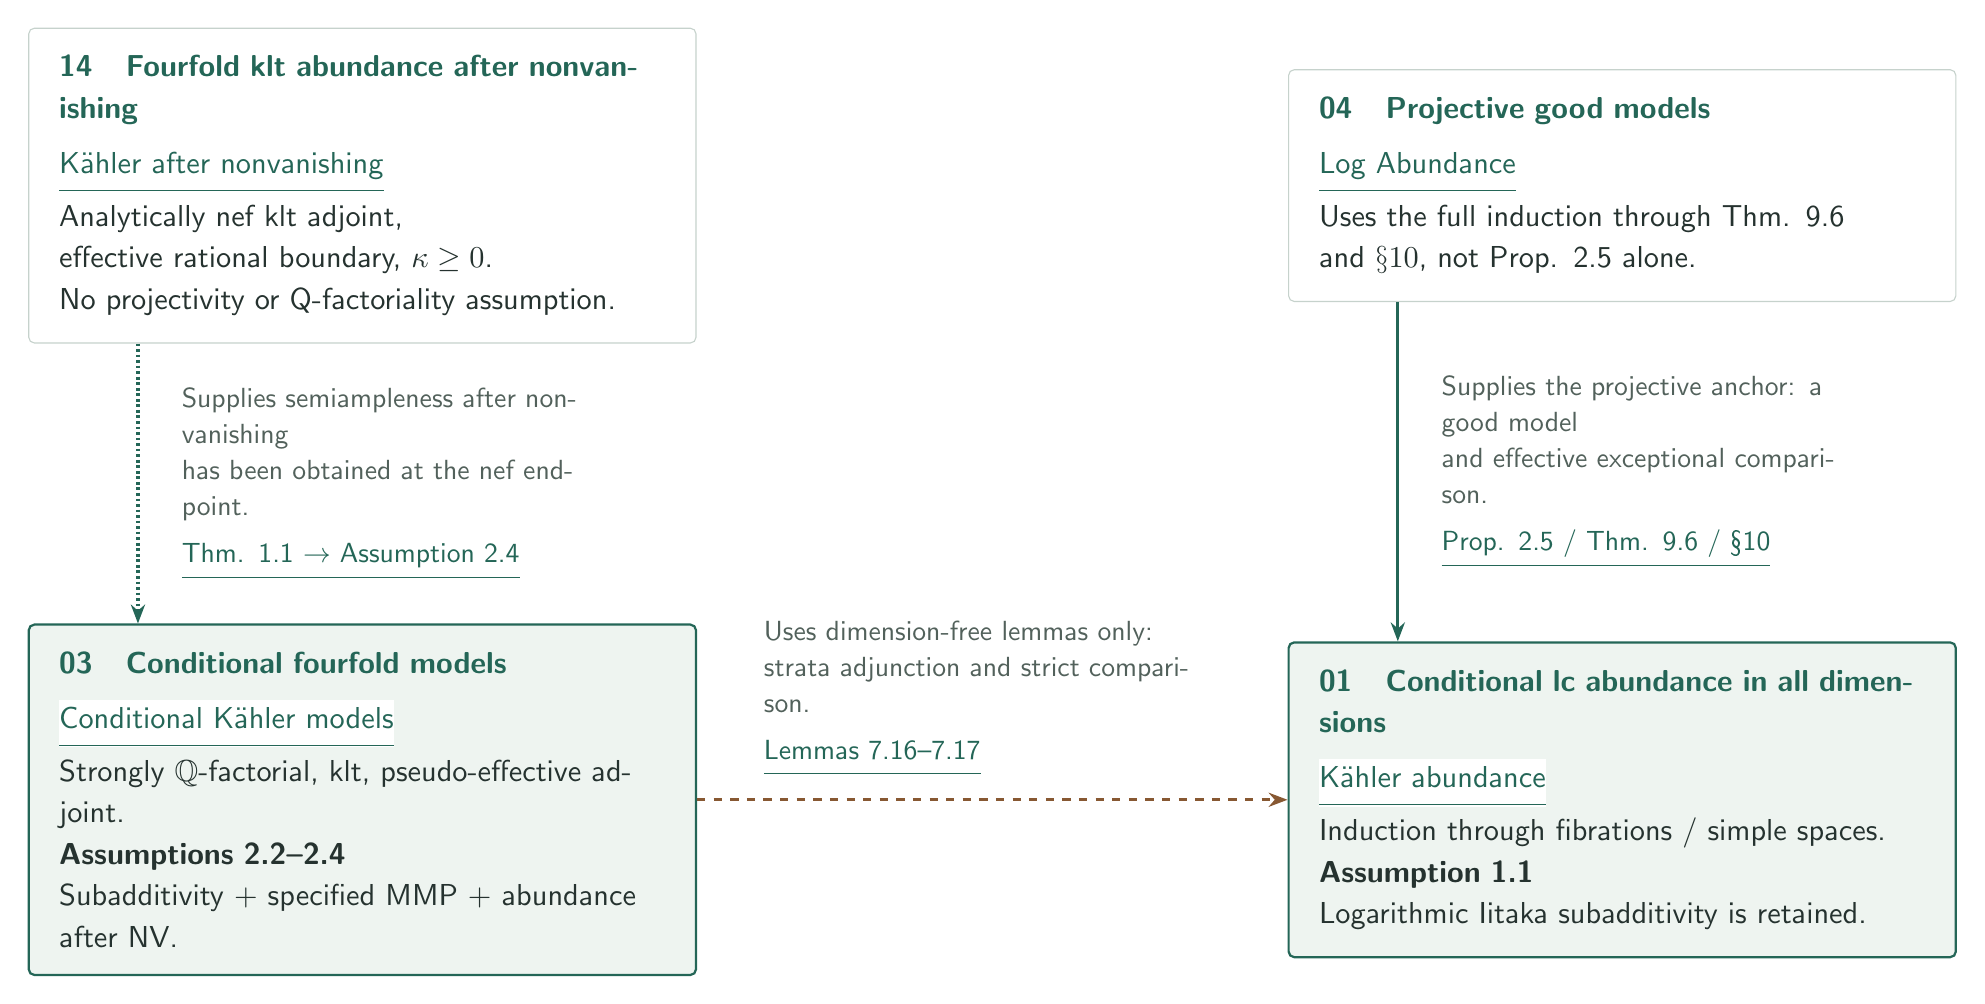
\begin{tikzpicture}
\node[card,text width=7.7cm] (after) at (0,0) {\Head{14\quad 非消滅後の四次元klt豊富性}{14\quad Fourfold klt abundance after nonvanishing}
\Paper{abundance-after-nonvanishing}{Kähler after nonvanishing}\\[4pt]
\Tx{解析的にnef、有効有理境界、$\kappa\ge0$。}{Analytically nef klt adjoint,\\effective rational boundary, $\kappa\ge0$.}\\
\Tx{射影性・Q-factorialityを仮定しない。}{No projectivity or Q-factoriality assumption.}};
\node[card,text width=7.7cm] (la) at (16,0) {\Head{04\quad 射影的な良いモデル}{04\quad Projective good models}
\Paper{log-abundance-characteristic-zero}{Log Abundance}\\[4pt]
\Tx{Prop. 2.5のみでなく、Thm. 9.6と\\$\S10$ までの帰納法全体を使う。}{Uses the full induction through Thm. 9.6\\and $\S10$, not Prop. 2.5 alone.}};
\node[result,text width=7.7cm,minimum height=3.2cm] (conditional) at (0,-7.8) {\Head{03\quad 条件付き四次元モデル}{03\quad Conditional fourfold models}
\Paper{conditional-kahler-fourfolds}{Conditional Kähler models}\\[4pt]
\Tx{strongly $\mathbb Q$-factorial、klt、擬有効随伴。}{Strongly $\mathbb Q$-factorial, klt, pseudo-effective adjoint.}\\
\textbf{Assumptions 2.2--2.4}\\
\Tx{劣加法性 + 指定MMP + 非消滅後の豊富性。}{Subadditivity + specified MMP + abundance after NV.}};
\Flow{after}{conditional}{premise}{\Tx{nef終点で非消滅を得た後に\\semiamplenessを供給。}{Supplies semiampleness after nonvanishing\\has been obtained at the nef endpoint.}\\[4pt]\Input{after-conditional}{Thm. 1.1 $\to$ Assumption 2.4}}
\node[result,text width=7.7cm,minimum height=3.2cm] (kahler) at (16,-7.8) {\Head{01\quad 全次元の条件付きlc豊富性}{01\quad Conditional lc abundance in all dimensions}
\Paper{kahler-log-abundance}{Kähler abundance}\\[4pt]
\Tx{ファイブレーション / simple空間の帰納。}{Induction through fibrations / simple spaces.}\\
\textbf{Assumption 1.1}\\
\Tx{対数飯高劣加法性を保持する。}{Logarithmic Iitaka subadditivity is retained.}};
\Flow{la}{kahler}{edge}{\Tx{射影的な良いモデルと\\有効例外比較を供給。}{Supplies the projective anchor: a good model\\and effective exceptional comparison.}\\[4pt]\Input{la-kahler}{Prop. 2.5 / Thm. 9.6 / \S10}}
\draw[auxiliary] (conditional.east)--(kahler.west);
\node[reason,text width=5.8cm,anchor=south] at (8,-7.5) {\Tx{次元制限のない補題だけを使用：\\strata随伴と厳密な比較。}{Uses dimension-free lemmas only:\\strata adjunction and strict comparison.}\\[4pt]\Input{conditional-kahler-strata}{Lemmas 7.16--7.17}};
\end{tikzpicture}

\end{document}
